
\documentclass[12pt,journal,compsoc]{IEEEtran}
\usepackage[nocompress]{cite}
\usepackage[cmex10]{amsmath}
\usepackage{algorithmic}
\usepackage{array}
\usepackage{mdwmath}
\usepackage{mdwtab}
\usepackage{eqparbox}
\usepackage[font=normalsize,labelfont=sf,textfont=sf]{subfig}
\usepackage{fixltx2e}
\usepackage{stfloats}
\usepackage{url}
\usepackage{graphicx}
\usepackage{arabtex}

\begin{document}
\title{Recognition-based Segmentation of On-line Handwritten Arabic Script}


\author{George~Kour,
		Raid~Saabne}


% The paper headers
%\markboth{Journal of \LaTeX\ Class Files,~Vol.~6, No.~1, January~2007}%
%{Shell \MakeLowercase{\textit{et al.}}: Bare Demo of IEEEtran.cls for Computer Society Journals}

%\IEEEspecialpapernotice{(Invited Paper)}


\IEEEcompsoctitleabstractindextext{%
\begin{abstract}
the handwritten form of the Arabic language raises some challenges for automatic character segmentation and recognition. Character segmentation is a fundamental part in many Optical Character Recognition (OCR) systems. However, Correct and efficient segmentation of Arabic text into characters is considered to be an essential problem. Its importance is derived from the fact that incorrectly segmented characters are unlikely to be recognized correctly. The Arabic script is composed of strokes which contain a single or multiple connected letters. In this paper, we propose a novel on-line strokes-level recognition-based segmentation technique of Arabic script. The uniqueness and the main contribution of our approach is that most time consuming parts are done while the stroke is being scribed. The system consists of three stages. The first stage requires the most calculation effort thus is performed whilst the stroke is being written and contains two parts, the first is rules based engine to determine candidate segmentation points based on topological features; the second part is recognition-based scoring of the subsequences induced by the nominated segmentation points. The second stage is filtering of the topologically invalid segmentation points. And the last stage is an algorithm which determines the best subset of segmentation points. The system has been designed and tested using the ADAB Database. Promising results are obtained without using context help.
\end{abstract}
\begin{IEEEkeywords}
Arabic Handwriting Recognition, Arabic Script Segmentation, Arabic Strokes Segmentation, On-line Text Recognition
\end{IEEEkeywords}}
\maketitle

\IEEEdisplaynotcompsoctitleabstractindextext

\section{Introduction}

\IEEEPARstart{H}{andwriting} remains the most used mean of communication and recording of information in the daily life. Therefore, a growing interest in the online character recognition field has taken place in the recent years.
Handwriting recognition (HWR) is a task of transforming a language represented in its spatial form of graphical marks into its symbolic representation. Handwriting recognition can be categorized into two main fields: on-line and off-line recognition. On-line handwriting recognition refers to the situation where the recognition is performed concurrently to the writing process. However, in the offline script recognition field, a digital image containing text is fed to the computers and the system attempt to recognize the written text \cite{al2011online}. The main existing approaches for script recognition are the holistic approach \cite{biadsy2011segmentation} and the analytic approach [add references]. The holistic approach considers the global properties of the written text while the analytic approach involves segmentation and classification of each part of the text.  In the holistic approach, the recognition system needs to be trained over all words in the dictionary, while it is possible for small vocabulary of words; this is not feasible for large vocabularies (20,000 words or more). Since each word is constructed from a subset of the character alphabet, it is much more efficient to classify words using the analytic approach. \cite{elanwar2012unconstrained}
The Arabic language is the fifth most used languages as a first language after Chinese, Hindi, Spanish and English. Around 350 million people use Arabic as their mother tongue. Most of them are citizens the Arab countries. Approximately 25 languages have adopted the Arabic alphabet slight some changes. Despite the fact that Arabic alphabets are used in many languages, the Arabic script recognition is at early stage in relation to the script recognition of Latin, Chinese and Kanji which has been a focus of study in the last decade and achieved an impressive recognition rates. The reason for this is mainly the difficulty in the nature of the Arabic script, lack of funds and other utilities such as text database, dictionaries, etc. \cite{zeki2011segmentation}
The Arabic language is written right to left in a cursive manner in both handwritten and printed forms. Some Arabic letters has 2 main body shapes: Isolated and final, while other letters have 4 main body shapes: Isolated, Final, Initial and Medial. An occurrence of two shapes letters inside a word will lead to a split of the body into two or more parts, called Word-Parts (WP). Within the WP, the letters are connected in both handwritten and printed. Different letters may share the same body and only differ by additional strokes and dots called delayed strokes. In many cases Arabic word parts, which are connected when printed, are written in different strokes in handwritten script. A stroke may contain a single or multiple connected letters and may represent the main letter body or a delayed stroke we have mentioned earlier.
 
\begin{figure}[h]
     \begin{center}
        \subfloat[]{
            \label{fig:kmbot_black}
            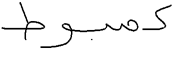
\includegraphics[width=0.2\textwidth]{./figures/kmbot_black}
        }
        \subfloat[]{
           \label{fig:kmbot_color}
           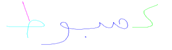
\includegraphics[width=0.2\textwidth]{./figures/kmbot_color}
        }        
    \end{center}
    \caption{
        The Tunisian city name kambot. As can be seen in (b) it contains two word parts (\RL{kmbw} and  \RL{.t}). The main body of the first word part is written in 2 strokes (\RL{k-} and \RL{-mbw}). The second WP contains only a single letter (\RL{.t}) and is written using 2 strokes, the main body and an additional stroke.   
     }
   \label{fig:kmbot}
\end{figure}

\begin{figure}[h]
     \begin{center}
        \subfloat[]{
            \label{fig:letters_same_body_1}
            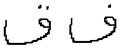
\includegraphics[width=0.2\textwidth]{./figures/letters_same_body_1}
        }
        \subfloat[]{
           \label{fig:letters_same_body_2}
           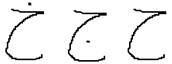
\includegraphics[width=0.2\textwidth]{./figures/letters_same_body_2}
        }        
    \end{center}
    \caption{
        Two letters groups which have the same main body and only differ by their additional strokes
     }
   \label{fig:same_main_body_letters}
\end{figure}

In the analytic approach, character segmentation is a crucial part of the text recognition process. Correct segmentation of a word into letter is likely to result in a correct recognition. The recognition-based segmentation approaches the other way around is also valid, a good recognition system improves the segmentation precision. Several segmentation techniques have been proposed in the literature for Arabic OCR. However correct and efficient segmentation of Arabic text is still considered a challenging and a fundamental problem even for off-line printed text.  
[talk about over and under segmentation in the general case, not specifically to the Arabic]
Restricting our discussion to the analytic approach, the segmentation can be classified two main methods
\begin{itemize}
  \item Dissection
  \item Recognition Based Segmentation
\end{itemize}
Dissection techniques learn the characteristic of the segmentation point and try to find these features in a candidate point. For example, in English cursive script segmentation a common feature is that segmentation point has local minima in the upper or lower contour of the word. Another feature is the slope of the segmentation point is low. Some techniques don't try to segment a word to its letters but to graphemes, which are a combination of 2 or 3 letters or is a part of a letter. The recognition-based techniques operation is quite different. In principle no feature-based dissection algorithm is employed. Rather, the image is divided systematically into many overlapping pieces without regard to content. These are classified as part of an attempt to find a coherent segmentation / recognition result. The main interest of this category of methods is that they bypass the segmentation problem: no complex "dissection" algorithm has to be built and recognition errors are basically due to failures in classification. In recognition-based techniques, recognition can be performed by following either a serial or a parallel optimization scheme. In the first case recognition is done iteratively in a left-to-right scan of words, searching for a "satisfactory" recognition result. The parallel method proceeds in a more global way. It generates a lattice of all (or many) possible feature-to-letter combinations. The final decision is found by choosing an optimal path through the lattice [2]. A common approach that is followed by many researchers is over-segmentation of the text and validating each such candidate segmentation point by extracting feature vectors representing the segmented parts to some classifier or rules based engine.\cite{daifallah2009recognition}

In this paper we propose a novel approach which performs segmentation and recognition in the strokes level. We combine both holistic and analytic techniques for recognizing open dictionary Arabic on-line script. In section 2 we mention related Work done in the field of online Arabic recognition. In section 3, we describe the details of our approach. Results are displayed in the section 4. We discuss and conclude the work in section 5.
\\ \emph{Decorate the Introduction by citations]}

\subsection{Related Work}
A rules-based system for off-line Arabic handwritten word segmentation was presented by Abdulla et al. in \cite{abdulla2008off}. Their method is based on extracting features of pixels lying on the upper contour. The freeman chain coding scheme was used to find the coordinates of the contour. The slope of the upper contour pixels is calculated and the direction of pairs of adjacent coordinate were marked by ‘+’ or ‘-‘. Segments were combined to formulate bigger decisive segments (DS). Set of possible segmentation point are nominated from the ‘+’ marked segments. These segmentation points were evaluated using a certain rules to find the final segmentation points (FSP). The system was tested on the demo version of IFN/INIT described in \cite{pechwitz2002ifn} , and their own AHD/AUST database.

Randa et al. proposed a two stage word segmentation system of online Arabic handwritten text based on Hidden Markov Model (HMM) \cite{elanwar2012unconstrained}. In the first stage, segmentation points were nominated by a simultaneous segmentation-recognition method using HMM.  The proposed segmentation points were validated by a rules-based stage. Additional strokes were removed and not taken into consideration in both parts. The system was tested using a self-collected database (OHASD) that was described in \cite{elanwar2010ohasd}.

Sari et al. in their paper \cite{sari2002off} proposed a method for off-line Arabic Word parts segmentation, based on the topological characteristics of the word contour. They applied 8-connected contour following algorithm to achieve a smoothed sequence of the X-Y coordinates of the outer contour. Then, identified Local minima in the lower outer contour to nominate Segmentation points and then formulated a rules based engine to identify valid segmentation points. The system was evaluated using a small database that contained 100 handwritten Arabic words sampled.

Laslo Digness et al. in \cite{Dinges2011} proposed a segmentation based recognition approach for off-line Arabic Handwritten words. Their method is based on dividing the word to smaller pieces which afterwards segmented into candidate letters and then classified into letter classes using statistical and structural features. Decisive tree were used to reduce the number of potential classes; neural networks to compute weights for all statistical features the output of this process was used as input for a k-NN classifier.

Khaled Daifallah et al. in \cite{daifallah2009recognition} proposed a method for on-line Arabic handwritten words recognition. Their method operates on the stroke level. It established on segmentation-based recognition which contain several stages. The first stage proposes over-segmentation of the stroke. The segmentation points are selected by locating semi-horizontal lines moving from right to left. In a latter phase a portion of the segmentation points is filtered out by applying on a certain set of rules. Then HMM is used to classify the sub-strokes to letters using Hu feature. The candidate and its scoring letters are obtained. Based on tis results the set of best segmentation points are selected.   


\subsection{Approach}
Subsection text here.

\section{Conclusion}
The conclusion goes here.

\bibliographystyle{IEEEtran}
\bibliography{IEEEabrv,bibliography}

\end{document}


